\section{Architecture}
 This section gives an overall view of the architecture and describes briefly the role of each component. A diagram summarising the architecture can be found in figure \ref{fig:architecture}

\subsection{Cothority}
The Omniledger project is part of the collective authority or Cothority project\cite{cothority}. Cothority is a framework for development, analysis and deployment of decentralised, distributed protocols. It is maintained and developed by the DEDIS lab at EPFL. The project's code is open source. Most Cothority projects are written in Java or Go, OmniLedger is written in the latter. \\\\
In Cothority, protocols are run on a given set of servers, called cothority servers or conodes, while the whole is referred to as a collective authority or cothority. In its current state, the project contains a few applications, such as ByzCoin, Onchain-Secrets and Proof of Personhood. \\\\
This project builds on top of ByzCoin, which already implements individual ledger with multiple transactions, a consensus protocol and smart contracts among other functionalities. In addition, the project also employs the ONet\cite{onet} and protobuf\cite{protobuf} packages. ONet or Overlay-network is the Cothority Network Library, it provides network abstraction functionalities to facilitate the deployment and test of decentralised protocols. Protobuf offers reflection-based protocol buffers, it allows the user to define message formats, encode and decode Go data structures. It is mainly used in inter-node communication.

\subsection{OmniLedger architecture}
In terms of architecture, an OmniLedger can be seen as a collection of ledgers composed of an identity ledger and several shard ledgers. To communicate with an OmniLedger, several components are required: A front-end client, an OmniLedger client and service, a ByzCoin client and service. In addition, smart contracts are also part of the architecture, as they define methods that can be executed on the ledgers.

\begin{figure}
	 \centering
	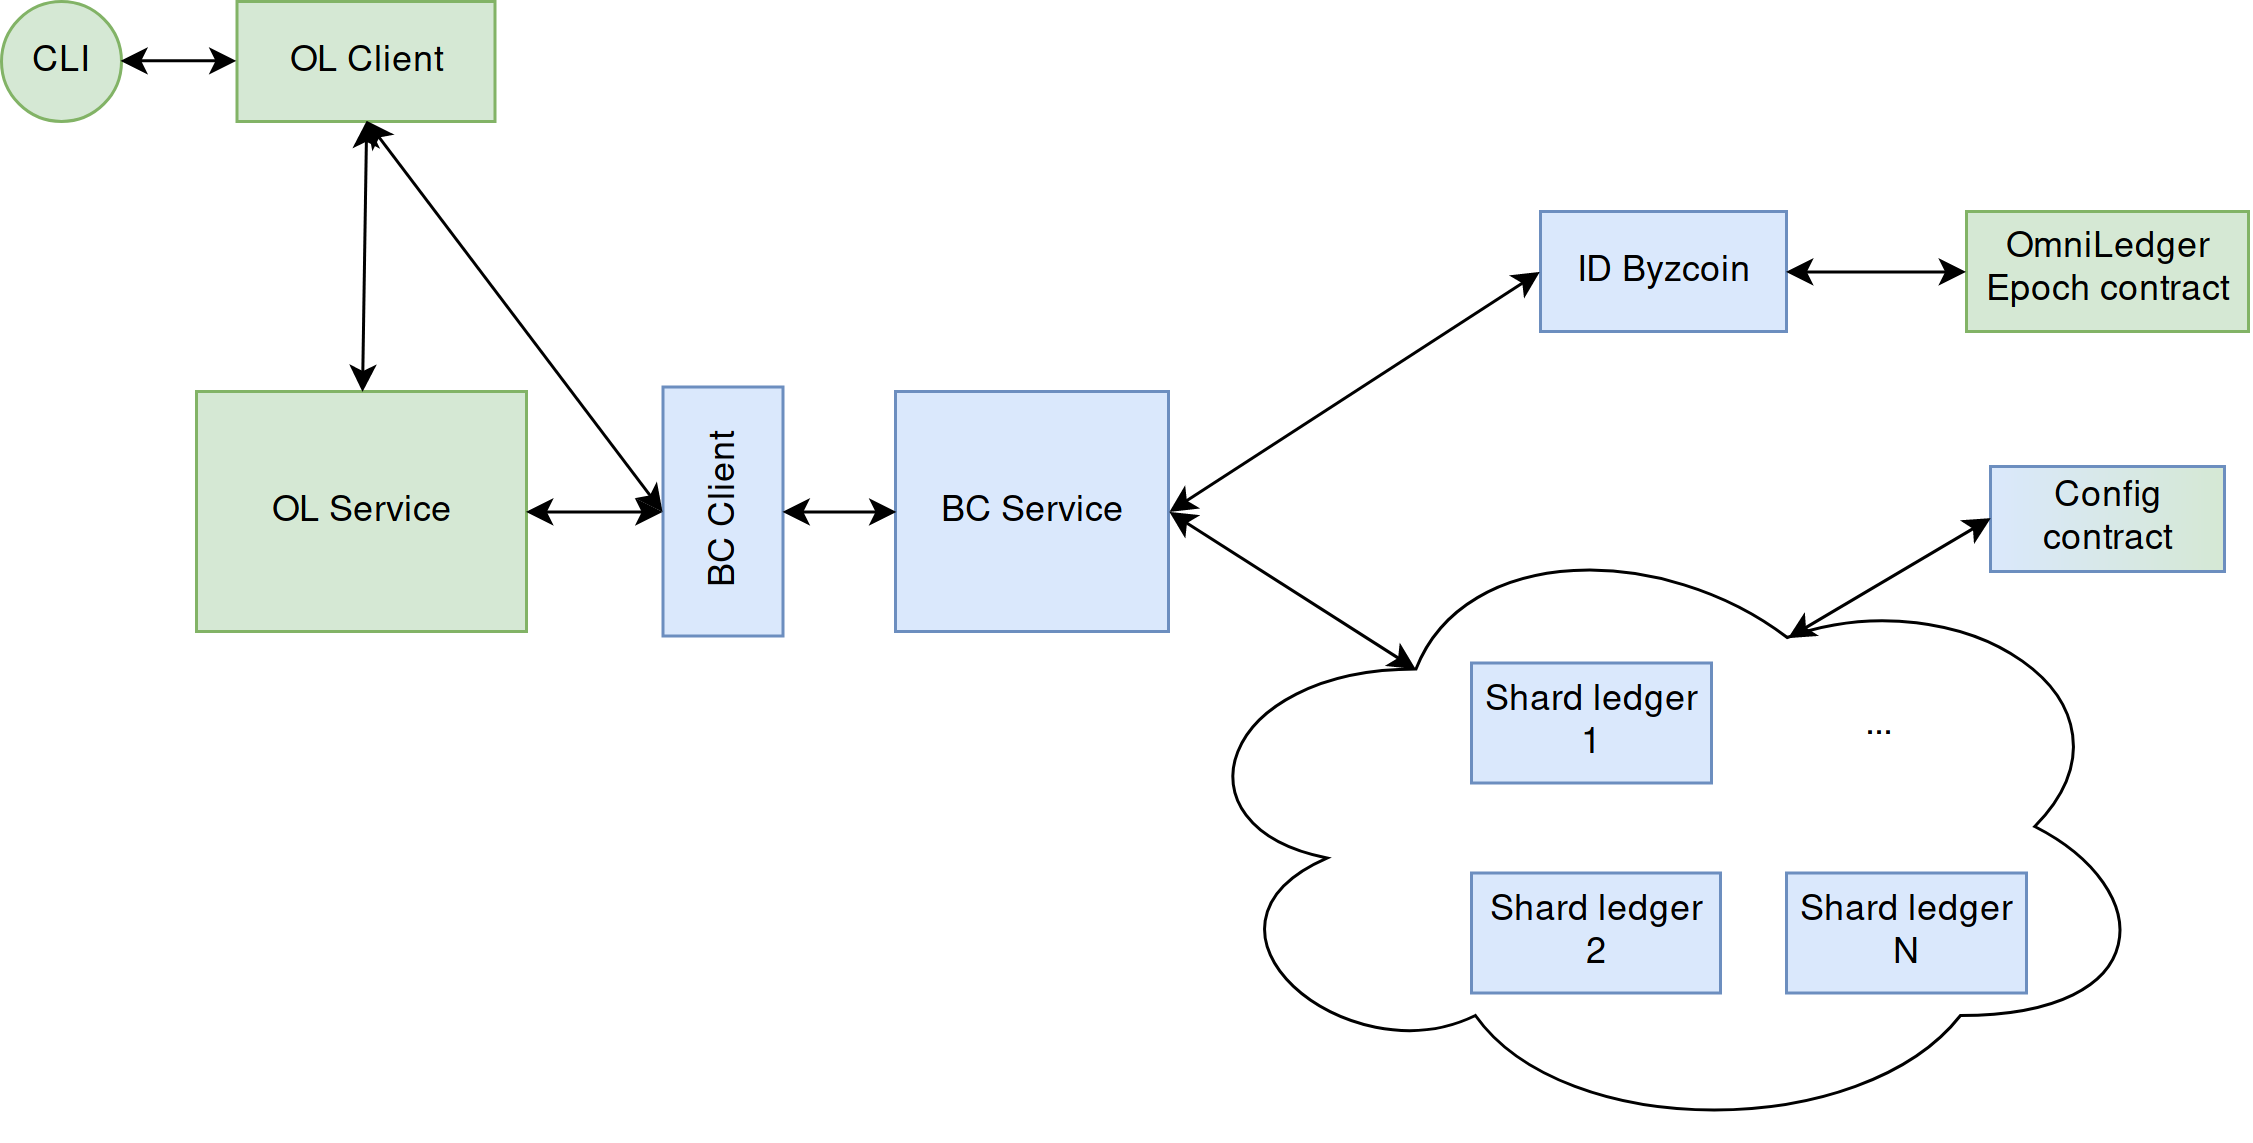
\includegraphics[width=\textwidth]{architecture.png}
	\caption{\label{fig:architecture} The OmniLedger architecture. Elements in green were implemented in this project. Elements in blue were already part of the Cothority framework. Config contract is in both colours as some code was added to it. The cloud of shard ledgers is used to abstract communication for every shard ledger, it is meant to imply that the BC service communicates with each shard ledger individually for example. }
\end{figure}

\subsubsection{Identity Ledger \& Shard ledgers}
The identity ledger, also referred to as identity ByzCoin or IB, has two responsibilities. The first is to keep track of nodes participating in the OmniLedger (often referred to as IB roster), as well as the roster of each shards. These two pieces of information, in addition to other configuration parameters (shard count, epoch size) are stored in the ledger state. The second is to compute the sharding assignment when the OmniLedger is created and in every subsequent new epochs.\\\\
A shard ledger is responsible for processing transactions. It also holds configuration information such as its roster, the maximum block size and the block interval. \\\\
Both the IB and the shard ledgers are implemented as ByzCoin ledgers. As a result, ByzCoin clients and the ByzCoin service must be used to communicate with them.

\subsubsection{CLI client}
The CLI (command-line interface) client serves as frontend for OmniLedger. It does some parameter checking before generating a request and sending it to OmniLedger service via the OmniLedger client. It was written with the help of the cli\cite{cli} package. The CLI is accessible via the \texttt{oladmin} executable. \\\\
At this moment, the following commands are available:
\begin{itemize}
	\item \texttt{oladmin create -shards <shard\_count> -epoch <epoch\_size> <roster\_file>} \\
	Creates a new OmniLedger with \texttt{<shard\_count>} shards and \texttt{ <epoch\_size>} epoch size. The command will generate two local \texttt{.cfg} files. The first contains the configuration of the created OmniLedger (roster of conodes, IB identity, shard identities, admin identity, etc). The second contains the ledger admin's keys.
	\begin{itemize}
		\item \texttt{<shard\_count>} should be low enough to form sufficiently large shards.
		\item \texttt{<epoch\_size>} is in milliseconds and indicates the minimum amount of time between two epochs.
		\item \texttt{<roster\_file>} is a \texttt{.toml} file containing the address, public key and a description of each participating conode. 
	\end{itemize}
	\item \texttt{oladmin newepoch <omniledger\_cfg> <key\_cfg>}\\
	Requests a new epoch for the OmniLedger specified by \texttt{<omniledeger\_cfg>}.
	\begin{itemize}
		\item \texttt{<omniledger\_cfg>} file holding the targeted OmniLedger configuration.
		\item \texttt{<key\_cfg>} file holding the keys of the admin of the targeted OmniLedger.
	\end{itemize}
	\item \texttt{oladmin status <omniledger\_cfg>}\\
	Prints the current OmniLedger roster and the shard rosters.
	\begin{itemize}
		\item \texttt{<omniledger\_cfg>} file holding the targeted OmniLedger configuration.
	\end{itemize}
\end{itemize}

\subsubsection{OmniLedger Client \& Service}
The OmniLedger service acts as an intermediate between the client and an OmniLedger. Its main role is to transform user requests into transactions to be sent to the ledgers. Its responsibilities include: 
\begin{itemize}
	\item Defining accepted user requests, their message structures and registering them.
	\item Processing user requests: checking parameter correctness, creating and sending the corresponding transactions, return response to the client.
	\item Coordinating the IB and the shard ledgers.
	\item Registering smart contracts.
\end{itemize}

\subsubsection{OmniLedger client}
The OmniLedger client is used to access with the OmniLedger service. It defines the API available from the front-end client. Even though in theory it should only forward requests to the OmniLedger service, in practice the client sometimes contact the ledgers directly.

\subsubsection{ByzCoin Client \& Service}
The ByzCoin service is used to communicate with the different shards composing an OmniLedger. It is part of the ByzCoin project, and thus was only used as a black-box for sending requests to the IB or the shard ledgers. Similarly to the OmniLedger service, the ByzCoin service is accessed by using a ByzCoin client.

\subsubsection{Smart Contract and Instances}
% Write about contracts in general
% Write about contracts in omniledger
OmniLedger and ByzCoin implement smart contracts. In short, they allow the definition of structures to be stored on the blockchain, as well as the definition of executable methods on these structures (more details on smart contracts and their implementation can be found in \cite{smart_contracts}). In this project, a new contract type was implemented: the OmniLedger Epoch contract. In addition, a new instruction was added to the Config contract of ByzCoin. \\\\
The OmniLedger Epoch contract stores an OmniLedger configuration as instance data, it contains the roster, the shard count, the epoch size, a timestamp and the shard rosters. The contract supports two instructions. The first is \texttt{spawn:omniledgerepoch}, it is used to set up a new OmniLedger. The second instruction is \texttt{invoke:request\_new\_epoch}, which is used to request a new epoch. More details on both instructions and how they are used in their respective context can be found in section \ref{ol-creation}  and \ref{new-epoch}.\\\\
The Config contract of Byzcoin was extended to support a new \texttt{invoke:new\_epoch} instruction. The execution of this instruction will compute the new shard roster and update the configuration.